\documentclass[a4paper,12pt]{article} 

%%% Работа с русским языком
\usepackage{cmap}                           % поиск в PDF
\usepackage{mathtext} 			 	       % русские буквы в формулах
\usepackage[T2A]{fontenc}               % кодировка
\usepackage[utf8]{inputenc}              % кодировка исходного текста
\usepackage[english,russian]{babel}  % локализация и переносы
\usepackage[left=2cm,right=2cm,
    top=2cm,bottom=2cm,bindingoffset=0cm]{geometry}

\usepackage{wrapfig}

\newcommand{\angstrom}{\mbox{\normalfont\AA}} % ангстрем

%Матеша
\usepackage{amsmath,amsfonts,amssymb,amsthm,mathtools, mathrsfs, wasysym}
\usepackage{icomma} % "Умная" запятая


%% Шрифты
\usepackage{euscript}	 % Шрифт Евклид


%%% Заголовок
\author{Гляудялис Гинтарас Б02-104}
\title{Лабораторная работа 4.1.2

Моделирование оптических приборов и определение их увеличения}
\date{\today}

\begin{document}

\maketitle

\begin{flushleft}
    \hspace*{2.5 mm}
    \textbf{Цели работы:}
    Определить фокусные расстояния собирающих и рассеивающих линз, 
    смоделировать ход лучей в трубе Галилея, трубе Кеплера и микроскопе, 
    определить их увеличение.\\
    \hspace*{2.5 mm}
    \textbf{В работе используются:}
    Оптическая скамья, набор линз, экран, осветитель со шкалой, 
    зрительная труба, диафрагма, линейка.
\end{flushleft}

\section*{Определение фокусных расстояний линз с помощью зрительной трубы}
\subsection*{Знакомство с линзами}
Рассмотрим доступные нам лизны и определим, какие из них являются собирающими, а какие --- рассеивающими. Для этого посветим параллельным пучком света через линзу и определим, наблюдается ли изображение (тогда линза положительная) и где (это будет фокус линзы). Для положительных также прикинем фокусное расстояние.
\par Получаем, что линзы 1-3 --- собирающие, а 4-5 --- рассеивающие. \par

\begin{enumerate}
    \item Настроим зрительную трубу на бесконечность
    \item Поставим положительную линзу на
расстоянии от предмета примерно равном фокусному. На небольшом расстоянии от линзы закрепим трубу, настроенную на бесконечность,
и отцентрируем её по высоте. Диафрагма диаметром
d = 1 см, надетая на ближнюю к осветителю линзу, уменьшит сферические аберрации и повысит чёткость изображения. \par
Передвигая линзу вдоль скамьи, получим в окуляре зрительной трубы изображение предмета
— миллиметровой сетки. При этом расстояние между предметом и серединой тонкой линзы (между проточками на оправах) равно фокусному.
    \item Результаты измерения фокусных расстояний собирающих линз:
\end{enumerate}
\begin{table}[h!]
	\caption{Фокусные расстояния собирающих линз}
	\begin{center}
		\begin{tabular}{|c|c|c|c|}
			\hline
			Сторона   & $ f_1,$ cм & $ f_2 $, см & $f_3 $, cм \\
			\hline
			Передняя &	 $8.3\pm0.5$	&	$10.4\pm0.5$   & $19.7\pm0.5$ \\
			\hline
			Задняя  &	$8.0\pm0.5$	&	$10.3\pm0.5$  & $19.8\pm0.5$ \\
			\hline
		\end{tabular}
	\end{center}
\end{table}

\subsection*{Определение фокусного расстояния рассеивающих линз}
\begin{enumerate}
    \item Для определения фокусного расстояния тонкой отрицательной линзы сначала получим на экране увеличенное изображение сетки при помощи одной короткофокусной положительной линзы. Измерим расстояние между линзой и экраном: $a_0 = 36.5$ см.
    \item Разместим сразу за экраном трубу, настроенную на бесконечность, и закрепим её. Уберём экран и поставим на его место исследуемую рассеивающую линзу (рис. 8). Перемещая рассеивающую линзу, найдём в окуляре зрительной трубы резкое изображение сетки. \par
    Измерив расстояние между линзами $l = 25.5$ см, рассчитаем фокусное расстояние рассеивающей линзы $f = a_0 - l$.
    \item Результаты измерения фокусного расстояния рассеивающих линз:
    \begin{center}
        $|f_5| = (11.0\pm0.5) $ см
    \end{center}
\end{enumerate}

\begin{figure}[h]
    \begin{center}
    \begin{minipage}[h]{0.45\linewidth}
    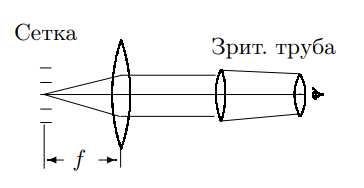
\includegraphics[width=1\linewidth]{plus_lens.PNG}
    \caption{Определение фокусного расстояния собирающей линзы} %% подпись к рисунку
    \end{minipage}
    \hfill 
    \begin{minipage}[h]{0.45\linewidth}
    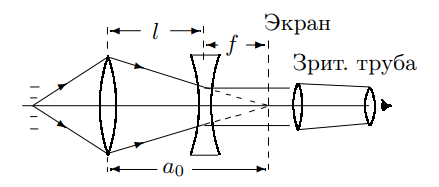
\includegraphics[width=1\linewidth]{minus_lens.PNG}
    \caption{Определение фокусного расстояния рассеивающей линзы}
    \end{minipage}
    \end{center}
    \end{figure}

\section*{Моделирование трубы Кеплера}
\begin{enumerate}
    \item Рассмотрим ход лучей в трубе Кеплера и найдём увеличение данной оптической системы:
    
\begin{figure}[h]
    \centering
    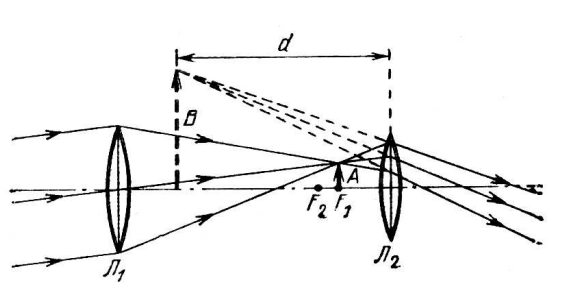
\includegraphics[width=9cm]{kepler.PNG}
    \caption{Ход лучей в трубе Кеплера}
\end{figure}

Пусть пучок света, попадающий в объектив, составляет с оптической осью угол $\varphi_1$, а пучок, выходящий из окуляра, — угол $\varphi_2$. Увеличение $\gamma$ зрительной трубы по определению равно
\begin{equation}
    \gamma = \frac{\tan \varphi_2}{\tan \varphi_1},
\end{equation}
но также из рис. 3 следует, что 
\begin{equation}
    \gamma_K = -\frac{f_1}{f_2} = -\frac{D_1}{D_2},
\end{equation}
где $D_1$ - ширина пучка, прошедшего через объектив, а $D_2$ - ширина пучка, вышедшего из окуляра

\item Построим оптическую систему из каллиматора и непосредственно трубы Кеплера. 

    \begin{figure}[h]
    \centering
    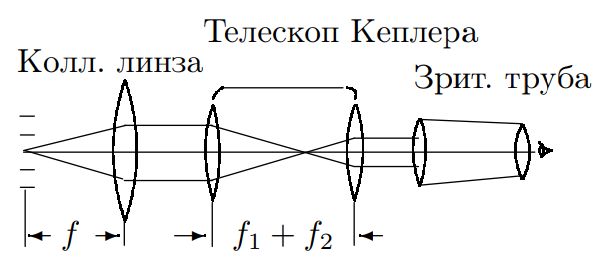
\includegraphics[width=9cm]{kepler_2.PNG}
    \caption{Схема трубы Кеплера}
\end{figure}

Параметры действующих линз:
\begin{center}
    $ f_1 = (8.3\pm0.5) $ см \hspace{1cm} $f_2 = (10.4\pm0.5) $ см
\end{center}

Найдём увеличение трубы Кеплера непосредственно: пусть $h_1$ - размер ячейки миллиметровой сетки без телескопа, $h_2$ - с телескопом
\begin{center}
$h_1 = (9 \pm 1)$ дел., \hspace{1cm} $h_2 = (11 \pm 1)$ дел.
\end{center}
\[\boxed{\gamma_K = -\frac{h_2}{h_1} = -1.2 \pm 0.2} \]

При этом по формуле (2) также
    \[ \boxed{\gamma_K = -\frac{f_1}{f_2} = -1.25 \pm 0.14} \] 


Полученные значения совпадают в пределах погрешности.
\end{enumerate}

\section*{Моделирование микроскопа}

\begin{figure}[h]
    \centering
    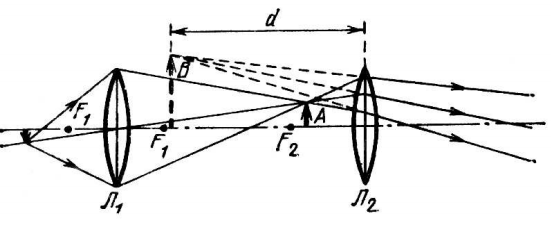
\includegraphics[width=9cm]{micro.PNG}
    \caption{Ход лучей в микроскопе}
\end{figure}

\begin{enumerate}
    \item Ход лучей в микроскопе показан на рис. 6. Увеличение микроскопа вычисляется по формуле
    \begin{equation}
        \gamma_M = \Gamma_{ob} \Gamma_{oc} = -\frac{\triangle}{f_1} \frac{L}{f_2},
    \end{equation}
    где $f_1$ и $f_2$ - фокусные расстояния линз микроскопа, $\triangle = l_{12}-f_1-f_2$ см - интервал, $ l_{12} $ -- длина тубуса, $L$ - расстояние наилучшего зрения ($L = 25$ см).
    
    \begin{figure}[h]
        \centering
        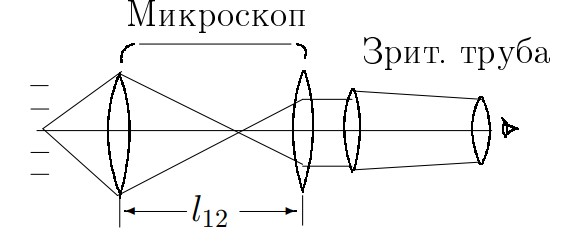
\includegraphics[width=9cm]{micro.jpg}
        \caption{Схема микроскопа}
    \end{figure}    
    
     Соберём микроскоп с пятикратным увеличением. Используемые линзы: $f_1 = 8.3 $ см, $ f_2 = 10.4 $ см. Получим
        \[ \gamma_M^\text{теор} = -\frac{\triangle}{f_1} \frac{L}{f_2} = -5 \]
    Исходя из этого получим необходимую длину тубуса $ l_{12} = 35.96 $ см.
    Проводя измерения угловых размеров миллиметровой сетки для такой конфигурации имеем $ h_2 = 35\pm1 $. Тогда
        \[ \boxed{\gamma_M^\text{эксп} = -\frac{h_2L}{h_1f} = -4.94 \pm 0.3} \]
        где $ f $ -- фокусное расстояние линзы-коллиматора из п.2, $ f = f_3 = 19.7 $ см.

Значения совпадают в пределах погрешности.
\end{enumerate}

\section*{Вывод}
В ходе выполнения лабораторной работы были получены следующие результаты:

\begin{itemize}
	\item Сначала при помощи поиска действительного изображения осветительного прибора в линзе было определен их тип. В итоге получилось, что линзы 1-3 -- собирающие, а 4-5 -- рассеивающие.
	\item В дальнейшем фокусное расстояние линз было определено при помощи зрительной трубы, настроенной на бесконечность. В итоге получаем следующие результаты:
	\begin{center}
		$f_1 = (8.1 \pm 0.6)$ см \hspace{1cm}  $f_2 = (10.4\pm0.6)$ см \hspace{1cm}  $f_3 = (19.8 \pm 0.6)$ см\hspace{1cm}  $f_5 = (-11.0 \pm 0.6)$ см
	\end{center}
	\item При моделировании оптических приборов было экспериментально измерено их увеличение, а затем сравнено с теоретическими значениями. Так, например, для трубы Кеплера имеем
	\[\gamma_K^\text{угл} = -\frac{h_2}{h_1} = -1.2 \pm 0.2 \]
	\[\gamma_K^\text{теор} = -\frac{h_2}{h_1} = -1.25 \pm 0.14 \]
	По результатам измерений можно сделать вывод о их совпадении в пределах погрешности.
	\item Также в ходе выполнения лабораторной работы была собрана модель микроскопа с планируемым теоретическим увеличением $  \gamma_M^\text{теор} = 5 $. В ходе эксперимента было получено следующее реальное значение увеличение микроскопа:
	\[ \gamma_M^\text{эксп} = -\frac{h_2L}{h_1f} = -4.94 \pm 0.3 \]
	Некоторое расхождение с теорией объясняется неточностью при выставлении приборов на оптической скамье, в особенности их продольных сдвигов.
\end{itemize}

\end{document}
